\chapter{Solver nonogramów}
\thispagestyle{chapterBeginStyle}

    W tym rozdziale opisany jest rozwój solvera. Opisane są kolejne główne wersje solverów. Zbadany
został także wpływ zastosowanych heurystyk na wydajność w rozwiązywaniu wybranych łamigłówek.



\section{Wersje solverów}


\subsection{Solver całościowy}
    Solver całościowy jest najprostszym z solverów implementowanych w toku pisania aplikacji. Jego
implementacja opiera się na założeniu, że obrazek ukryty w łamigłówce jest ciągiem pustych i pełnych
pikseli. Solver sprawdza wszystkie możliwe kombinacje pól, aż do wykrycia rozwiązania, bądź stwierdzenia
jego braku. Wskazówki umieszczone obok planszy służą jedynie do walidacji rozwiązania, i nie są
wykorzystywane w trakcie rozwiązywania nonogramu.

\begin{figure}[!htb]
    \centering
    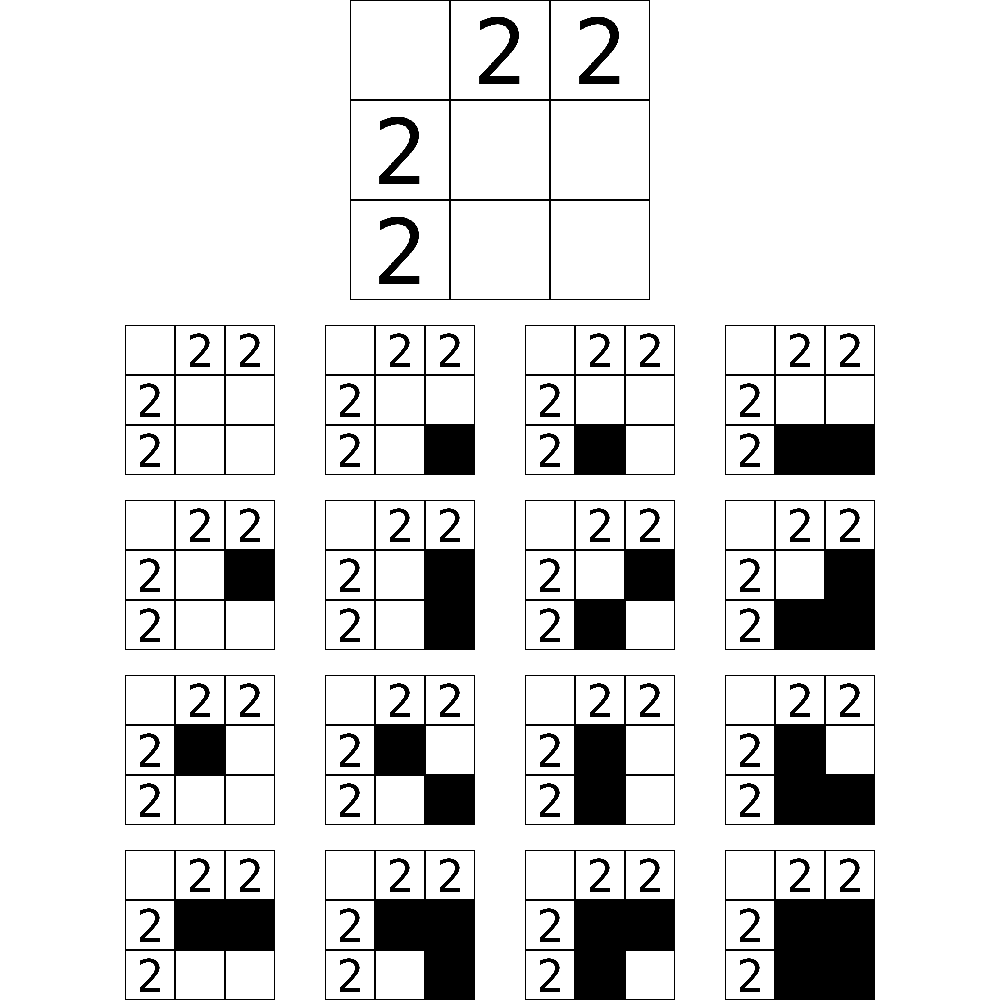
\includegraphics[width=0.5\textwidth]{images/all_solver_example.png}
    \caption{Solver całościowy sprawdza wszystkie możliwe układy planszy w celu znalezienia rozwiązania.}
\end{figure}

    Solver ten zaczyna od pustej planszy. Następnie, dla pierwszego pola wywoływana jest rekursyjna
metoda: jeśli indeks pola mieści się w zakresie planszy, to najpierw jego status ustawiany jest na
pusty, i następuje wywołanie metody dla nastepnego indeksu, a jeśli rozwiązanie nie zostanie znalezione,
to pole jest wypełniane i ponownie dochodzi do wywołania metody na następnym polu. Jeśli indeks
wykracza poza zakres planszy, to znaczy że wszystkie pola mają ustawiony status i wywoływana jest
metoda sprawdzająca poprawność rozwiązania, podobna do tej opisanej w \ref{alg:axisValidation}.
Jeśli solver zakończy działanie zwracając \texttt{true}, to w przekazanej mu macierzy pól 
(równoznaczne z listą wierszy) znajdzie się rozwiązanie łamigłówki.

\begin{pseudokod}[H]
    %\SetAlTitleFnt{small}
    \SetArgSty{normalfont}
    \SetKwFunction{Verify}{Verify}
    \KwIn{Lista wierszy $R$, indeks pola $i$, lista wskazówek wierszy $Hr$ i kolumn $Hc$, szerokość $w$ i wysokość $h$ planszy}
    \KwOut{Czy znaleziono rozwiązanie \texttt{true/false}}
    \If{$i \geq w \cdot h$}{
        \texttt{return} \Verify{$R$, $Hr$, $Hc$, $w$, $h$}\;
    }
    \Else{
        $iWiersza \leftarrow \lceil \frac{i}{w} \rceil$\;
        $iKolumny \leftarrow i\ mod\ w$\;
        $R[iWiersza][iKolumny] \leftarrow 0$\;
        \If{\texttt{SolverCałościowy}($R, i+1, Hr, Hc, w, h$)}{
            \texttt{return true}\;
        }
        $R[iWiersza][iKolumny] \leftarrow 1$\;
        \texttt{return SolverCałościowy}($R, i+1, Hr, Hc, w, h$)\;
    }
    \caption{SolverCałościowy}\label{alg:allSolver}
\end{pseudokod}

    Złożoność czasowa tego solvera jest bardzo duża. Procedura sprawdzająca poprawność rozwiązania
może zostać wywołana $2^{w*h}$ razy, czyli inaczej $2^n$, gdzie $n$ to ilość pól na planszy. 
Wynika to z faktu, że kazde kolejne pole wymaga sprawdzenia pól poprzednich, a samo może znajdować
się w dwóch stanach, więc podwaja ilość wywołań procedury sprawdzającej.


\subsection{Solver osiowy}
    W odróżnieniu od solvera całościowego, solver osiowy korzysta ze wskazówek przy szukaniu rozwiązań.
Opiera się on na fakcie, że każda linia (wiersz lub kolumna) może znajdować się w jednym z możliwych
stanów, których liczba nigdy nie dojdzie do $2^x$, gdzie $x$ jest długością linii. Sprawdzając
rozwiązanie w tym solverze, gwarantowana jest poprawność w jednej z osi, co dodatkowo znacząco skraca
czas szukania rozwiązania.

\begin{figure}[!htb]
    \centering
    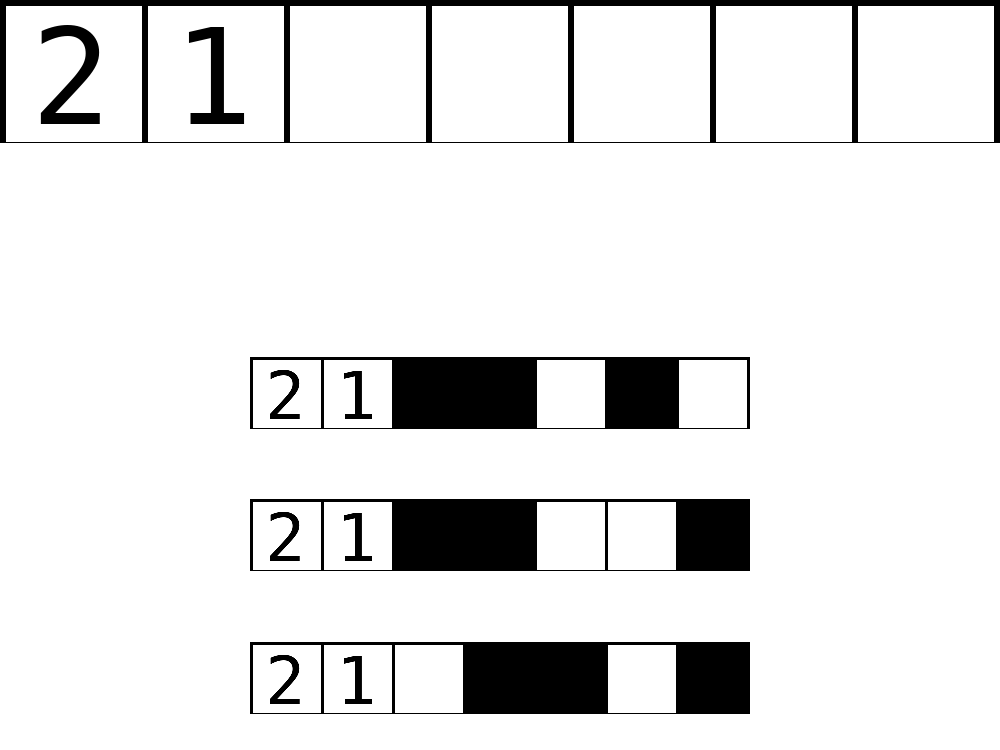
\includegraphics[width=0.5\textwidth]{images/axis_solver_example.png}
    \caption{Dla linii na grafice, solver osiowy spradza jedynie 3 stany. Dla tej samej linii,
solver całościowy sprawdziłby $2^5 = 32$ stany
    }
\end{figure}

    Solver zaczyna od pustej planszy. Przed rozpoczęciem rozwiązywania sprawdzana jest ilość wszystkich
kombinacji w danej osi (iloczyn możliwości każdej z linii), i wybierana jest oś z mniejszą liczbą
możliwości. Następnie generowane są kombinacje dla każdej z linii. Solver korzysta z rekursyjnej
metody, i ustawia pierwszą kombinację dla pierwszej linii. Następnie wywołuje metodę dla kolejnej linii,
aż do ostatniej, i wtedy weryfikuje rozwiązanie. Jeśli dla danego ustawienia w linii łamigłówka
nie ma rozwiązania, to solver przechodzi do kolejnego ustawienia i wywołuje metodę w kolejnej linii.

\begin{pseudokod}[H]
    %\SetAlTitleFnt{small}
    \SetArgSty{normalfont}
    \SetKwFunction{Verify}{Verify}
    \SetKwFunction{NalozKombinacje}{NalozKombinacje}
    \KwIn{Lista linii $L$, indeks linii $i$, lista wskazówek linii prostopadłych $H$, ilość linii $n$}
    \KwOut{Czy znaleziono rozwiązanie \texttt{true/false}}
    \If{$i = n$}{
        \texttt{return} \Verify{$L$, $H$, $n$}\;
    }
    \Else{
        $linia \leftarrow L[i]$\;
        \ForEach{$komb \in linia.kombinacje$}{
            \NalozKombinacje{$linia, komb$}\;
            \If{\texttt{SolverOsiowy}($L, i+1, H, n$)}{
                \texttt{return true}\;
            }
        }
        \texttt{return false}\;
    }
    \caption{SolverOsiowy}\label{alg:axisSolver}
\end{pseudokod}

    Dzięki eliminacji kombinacji sprzecznych ze wskazówkami w danej osi, procedura sprawdzania
poprawności rozwiązania jest wywoływana o wiele rzadziej niż w przypadku solvera całościowego.
O ile ilość kombinacji w linii przy rozpatrywaniu każdej komórki z osobna to $2^n$, gdzie $n$ to
długość linii, tak w przypadku rozważania poprawnych kombinacji dla linii jest ona zależna od
długości i zawartości wskazówki, i można ją ograniczyć z góry przez
${n + 1 - h} \choose h$, a $h$ to ilość wskazówek w linii. To przybliżenie jest zawyżone, ponieważ
zakłada występowanie jedynie bloków długości jeden we wskazówce. W przeciętnym przypadku, bloki
wypełnionych komórek będą dłuższe, oraz będzie ich mniej. Dodatkowo, jak zostało wspomniane na początku,
weryfikacja jest wymagana jedynie w jednej z dwóch osi, jako że konstrukcja potencjalnych rozwiązań
opiera się o zestawianie poprawnych kombinacji z linii.


\subsection{Solver eliminacyjny}
    Solverem, którego wariant znajduje się w aplikacji, jest solver eliminacyjny. W przeciwieństwie
do wcześniej opisanych solverów, solver ten nie zakłada układów komórek w liniach tak długo jak to
możliwe. W jego wypadku, generowane są możliwe kombinacje dla każdej z linii (zarówno wierszy jak i
kolumn). W danym przejściu eliminowane są kombinacje sprzeczne z dostępnymi informacjami 
(np. kombinacje posiadające pełną pierwszą komórkę, podczas gdy pewne jest że jest ona pełna) 
oraz wyciągane są części wspólne kombinacji (np. wszystkie kombinacje mają pustą drugą komórkę), 
które dostarczają informacji dla innych linii. Dodatkowo, w przeciwieństwie do poprzednich solverów,
nie jest konieczna walidacja rozwiązania, jako że rozwiązanie jest poprawne w momencie, gdy każdy
wiersz i każda kolumna ma dostępną jedną możliwą komibnację.

\begin{figure}[!htb]
    \centering
    \begin{subfigure}[b]{0.35\textwidth}
        \centering
        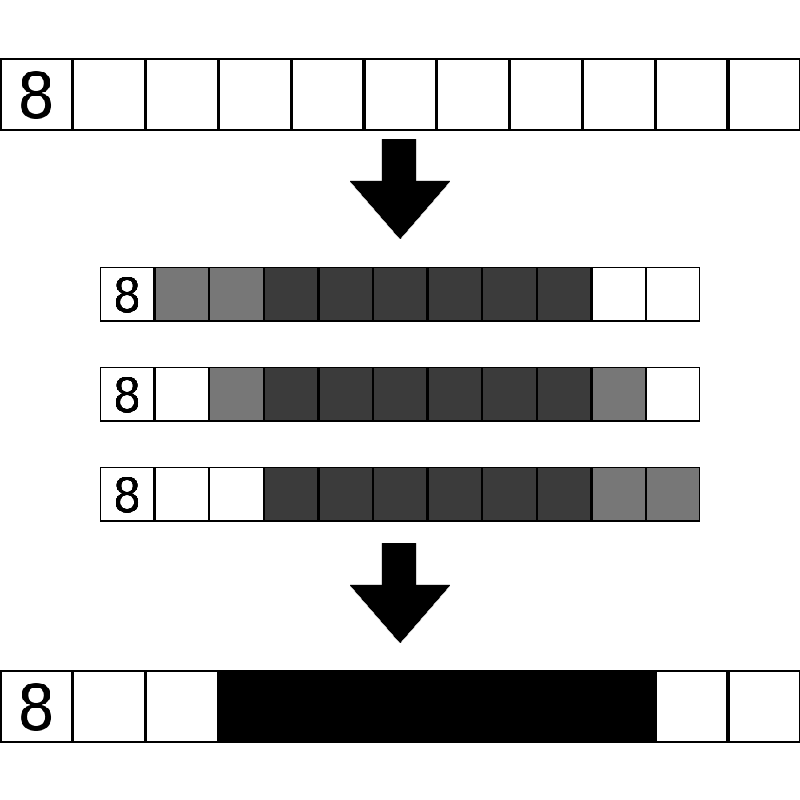
\includegraphics[width=\textwidth]{images/elimination_solver_example_a.png}
        \caption{pola wspólne dla wszystkich kombinacji zostają naniesione na planszę}
    \end{subfigure}
    \hspace{0.1\textwidth}
    \begin{subfigure}[b]{0.35\textwidth}
        \centering
        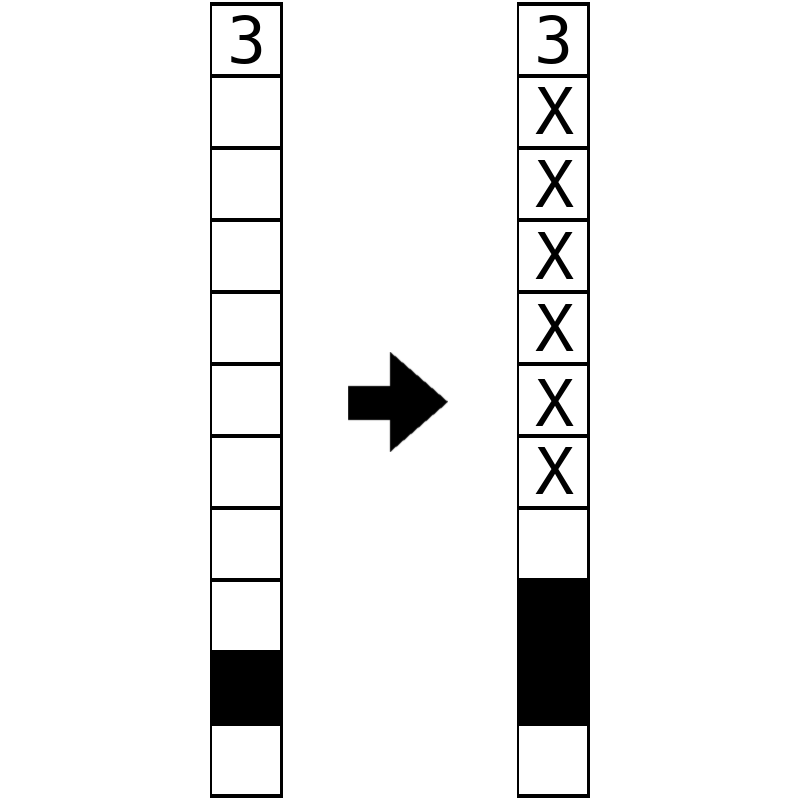
\includegraphics[width=\textwidth]{images/elimination_solver_example_b.png}
        \caption{korzystając z informacji z wiersza, solver wnioskuje stan większości pól w kolumnie
        (x oznacza pole definitywnie puste)}
    \end{subfigure}
    \caption{Przykład wnioskowania na podstawie możliwych kombinacji}
\end{figure}

    Solver zaczyna od pustej planszy. Na początku generowane są wszystkie kombinacje dla każdej z
linii, a linie wrzucane są do kolejki \textit{last-in first-out}. Następnie solver przechodzi do
rozwiązywania. Dopóki kolejka nie jest pusta, to są linie, których komibnacje należy zweryfikować.
Z kolejki usuwana jest sprawdzana linia. Dla tej linii następują dwa kroki: najpierw, eliminowane
są kombinacje sprzeczne z układem danej linii. W wypadku tego solvera, każda komórka znajduje się
w jednym z trzech stanów: \textit{pełny}, \textit{pusty} i \textit{nieznany}. Stan \textit{nieznany}
komórki dopuszcza kombinacje zawierające komórkę pełną lub pustą; pozostałe stany wymagają
zgodności stanu ze stanem komórki w kombinacji. Po eliminacji sprzecznych kombinacji, dochodzi
do porównania kombinacji. Jeśli istnieje komórka w linii, której stan jest \textit{nieznany}, a
wszystkie pozostałe kombinacje mają ustawiony dla niej ten sam stan, to stan komórki jest aktualizowany,
a prostopadła linia zostaje dodana do kolejki do weryfikacji (następuje przy tym upewnienie, że
w kolejce nie ma powtórzeń). Kiedy kolejka zostanie opróżniona, sprawdzane są linie.
Jeśli wszystkie linie mają jeden możliwy stan, to znaczy że zostało znalezione rozwiązanie. Jeśli
któraś z linii nie ma możliwej kombinacji, to nie istnieje rozwiązanie przy dokonanych założeniach.
W przeciwnym wypadku, solver zakłada poprawność jednej z kombinacji dla linii
o kilku możliwych kombinacjach. Jako że wskutek założenia stan linii zmienił się, to do kolejki
dodawane są linie prostopadłe. Następnie wywoływana jest w sposób rekursyjny metoda rozwiązująca
nonogram dla obecnego stanu planszy. Jeśli rozwiązanie nie zostanie znalezione w tej gałęzi, to
solver zakłada poprawność kolejnej kombinacji dla tej linii.

\begin{pseudokod}[H]
    %\SetAlTitleFnt{small}
    \SetArgSty{normalfont}
    \SetKwFunction{SprawdzLinie}{SprawdzLinie}
    \SetKwFunction{NalozKombinacje}{NalozKombinacje}
    \SetKwFunction{UzupelnijKolejke}{UzupelnijKolejke}
    \KwIn{Lista wierszy $R$ i kolumn $C$, kolejka $Q$}
    \KwOut{Czy znaleziono rozwiązanie \texttt{true/false}}
    \While{$Q.zawieraElementy()$}{
        $linia \leftarrow Q.pop()$\;
        \SprawdzLinie{$linia$}\;
    }
    \If{$(\forall linia \in R \bigcup C)(|linia.kombinacje| = 1)$}{
        \texttt{return true}\;
    }
    \uElseIf{$(\exists linia \in R \bigcup C)(|linia.kombinacje| = 0)$}{
        \texttt{return false}\;
    }
    \Else{
        $zakladanaLinia \leftarrow$ pierwsza linia z wieloma kombinacjami\;
        \ForEach{$komb \in zakladanaLinia.kombinacje$}{
            $kopiaR \leftarrow kopiuj(R)$\;
            $kopiaC \leftarrow kopiuj(C)$\;
            \NalozKombinacje{$zakladanaLinia, komb$}\;
            \UzupelnijKolejke{$Q$}\;
            \If{\texttt{SolverEliminacyjny}($kopiaR, kopiaC, Q$)}{
                $R \leftarrow kopiaR$\;
                $C \leftarrow kopiaC$\;
                \texttt{return true}\;
            }
        }
        \texttt{return false}\;
    }
    \caption{SolverEliminacyjny}\label{alg:eliminationSolver}
\end{pseudokod}

\begin{pseudokod}[h]
    %\SetAlTitleFnt{small}
    \SetArgSty{normalfont}
    \SetKwFunction{WeryfikujKombinacje}{WeryfikujKombinacje}
    \KwIn{Linia $l$}
    \ForEach{$komb \in l.kombinacje$}{
        \If{\texttt{!WeryfikujKombinacje}($l$)}{
            $l.kombinacje.usun(l)$\;
        }
    }
    \ForEach{$i \in \{1, 2, \ldots, |l|\}$}{
        \If{$l[i] =$ \textit{nieznany} $\land$ pole identyczne we wszystkich kombinacjach}{
            $l[i] = $ nowy stan\;
            $Q.dodaj$(linia prostopadła do $l$ o indeksie $i$)\;
        }
    }
    \caption{SprawdzLinie}\label{alg:eliminationSolver_checkLine}
\end{pseudokod}

    Istotna uwaga dotyczy charakterystyki wierszy i kolumn. W celu umożliwienia działania procedury
został wykorzystany mechanizm obecny w wielu powszechnie używanych językach programowania, mianowicie
mechanizm płytkiej kopii. Mimo że listy wierszy i kolumn zawierają inne obiekty (listy), to obiekty
komórek przechowywane w tych zagnieżdżonych listach są takie same. Dzięki temu, modyfikując stan
komórki w liście wierszy w $n$-tym wierszu i $m$-tej komórce, modyfikujemy także stan komórki
zawartej w $n$-tej komórce w $m$-tej kolumnie w liście kolumn.



\section{Porównanie wydajności solverów}
    W tej części zbadane zostały wydajności poszczególnych wersji solverów oraz wpływ wybranych
modyfikacji i heurystyk na ich wydajność.


\subsection{Metodyka badań}
    Metoda prowadzenia badań jest następująca: dla każdej łamigłówki prowadzonych jest 5 prób 
rozwiązania. Próby z minimalnym oraz maksymalnym czasem rozwiązywania zostają odrzucone, w celu
eliminacji błędów powstałych na skutek zaburzeń występujących w trakcie prowadzenia testu. Następnie
czas pozostałych 3 prób zostaje uśredniony i podany jako wynik badania. Jeśli czas wykonania
iteracji testu przekroczy 5 minut, to test zostaje przerwany i do komórki zostaje wpisany wynik
\textit{przekroczono}.

    Testy zostały przeprowadzone na komputerze z procesorem Intel Core i5-6300HQ, z
16GB pamięci RAM o taktowaniu 2133Mhz. Testy zostały uruchomione w środowisku Node.js \cite{node}
w wersji v14.18.2. Czas rozwiązywania łamigłówek na urządzeniu mobilnym może znacząco odbiegać
od czasów zaprezentowanych w wynikach, z powodu mniejszych zasobów i zastosowanego środowiska
uruchomieniowego.

    Wyniki zostały zaprezentowane w tabelach o następującym układzie: w pierwszych dwóch kolumnach
zostały podane nazwy łamigłówek i ich wielkości (łamigłówki są zadane na planszach kwadratowych).
W kolejnych kolumnach, nazwanych odpowiednio do zastosowanej modyfikacji bądź jej braku,
podany jest czas rozwiązywania nonogramu wyrażony w milisekundach. Czas jest zaokrąglony do pełnych
milisekund, zatem dla prostych łamigłówek może być wyrażony jako 0.

    Zestaw danych użyty do testów został przedstawiony na końcu rozdziału.


\subsection{Solver całościowy}
    Wydajność solvera całościowego została sprawdzona na zestawie 4 łamigłówek.

\subsubsection{Wyniki}
\begin{table}[h]
    \begin{center}
        \begin{tabular}{|c|c|r|}
            \hline
            Nazwa          & Rozmiar        & Czas rozwiązywania w ms \\
            \hline
            Cross       & 3 & 1                     \\
            Flame       & 5 & 46                    \\
            Jellyfish   & 8 & \textit{przekroczono} \\
            Candy       & 8 & \textit{przekroczono} \\
            \hline
        \end{tabular}
    \end{center}
    \caption{Wyniki testów dla solvera całościowego}
\end{table}

\subsubsection{Interpretacja}
    Solver całościowy jest w stanie dość szybko rozwiązać niewielkie łamigłówki,
ale czas jego pracy rośnie bardzo szybko wraz ze wzrostem wielkości planszy.


\subsection{Solver osiowy}
    Wydajność solvera całościowego została sprawdzona na pełnym zestawie 18 łamigłówek. Został
on poddany jednej modyfikacji.

\subsubsection{Modyfikacje}
    \textbf{Częściowa weryfikacja} rozwiązania polega na wykorzystaniu procedury częsciowej weryfikacji.
Jest ona podobna do procedury weryfikacji w osi, ale nie sprawdza poprawności całej planszy,
a jedynie sprawdza czy dany układ może prowadzić do poprawnego rozwiązania (czyli czy nie ma sprzeczności na tym etapie).
Procedura otrzymuje głębokość dla jakiej ma zweryfikować poprawność. Jeśli do danej głębokości nie
występuje sprzeczność, to rozwiązanie jest konstruowane dalej. W przeciwnym przypadku, w danej gałęzi
nie może być poprawnego rozwiązania, i solver przechodzi do innej gałęzi.

\begin{figure}[!htb]
    \centering
    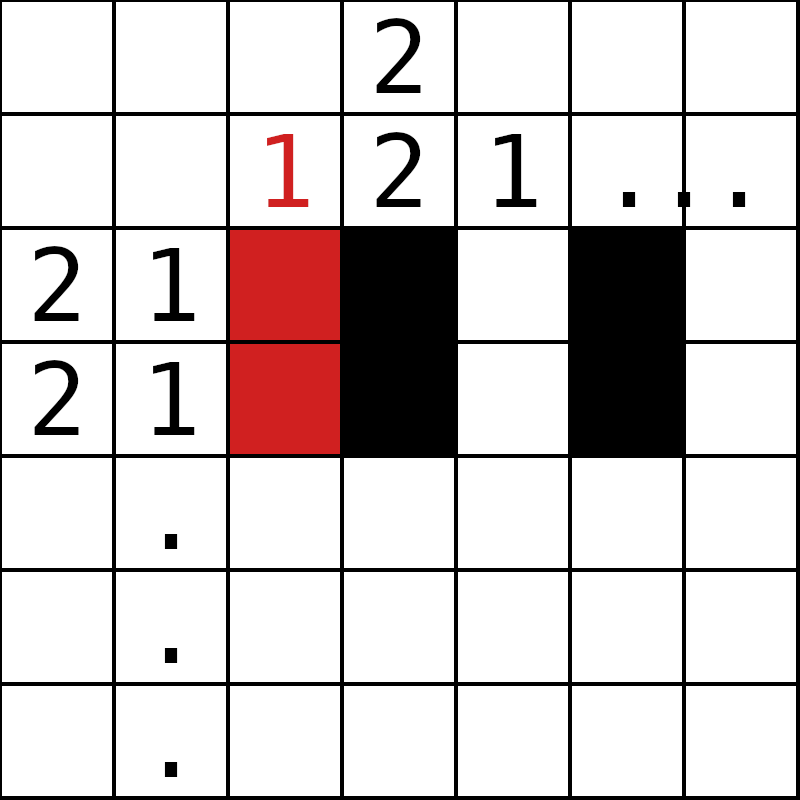
\includegraphics[width=0.4\textwidth]{images/partial_check_example.png}
    \caption{Na tym etapie można zdyskwalifikować każde rozwiązanie zawierające pierwszy i drugi wiersz
w układzie widocznym na grafice}
\end{figure}



\subsubsection{Wyniki}
\begin{table}[h!]
    \begin{center}
        \begin{tabular}{|c|c|r r|}
            \hline
            {}          & {}        & \multicolumn{2}{c|}{Czas rozwiązywania w ms} \\
            Nazwa       & Rozmiar   & bez modyfikacji & z częściową weryfikacją \\
            \hline
            Cross       & 3         & 0                     & 0 \\
            Flame       & 5         & 0                     & 0 \\
            Jellyfish   & 8         & 463                   & 2 \\
            Candy       & 8         & 0                     & 0 \\
            Shield      & 10        & \textit{przekroczono} & 3 \\
            Dog         & 10        & 12004                 & 1 \\
            Duck        & 16        & \textit{przekroczono} & 12 \\
            Shrimp      & 16        & \textit{przekroczono} & 14 \\
            Cherries    & 20        & \textit{przekroczono} & 25 \\
            Potion      & 20        & \textit{przekroczono} & 315 \\
            Tape        & 25        & \textit{przekroczono} & 1091 \\
            Lighter     & 25        & \textit{przekroczono} & 60945 \\
            \hline
            Ghost       & 32        & \textit{przekroczono} & 40040 \\
            Demon       & 32        & \textit{przekroczono} & 3997 \\
            Butcher     & 48        & \textit{przekroczono} & \textit{przekroczono} \\
            Ranger      & 48        & \textit{przekroczono} & 59703 \\
            Orc         & 64        & \textit{przekroczono} & \textit{przekroczono} \\
            Swordsman   & 64        & \textit{przekroczono} & \textit{przekroczono} \\
            \hline
        \end{tabular}
    \end{center}
    \caption{Wyniki testów dla solvera osiowego}
\end{table}

\subsubsection{Interpretacja}
    W podstawowej wersji, solver osiowy ma niewiele lepszą wydajność od solvera całościowego,
będąc w stanie rozwiązać niektóre łamigłówki wielkości 10 przy nałożonym ograniczeniu czasowym. 
Jednak po dodaniu częsciowej weryfikacji, wydajność solvera drastycznie wzrasta, i może zostać
wykorzystany do rozwiązywania łamigłówek o wiele większych niż w przypadku podstawowej wersji.
Pokazuje to jak kluczowa jest wstępna eliminacja niepożądanych gałęzi przy rozwiązywaniu danego
problemu.


\subsection{Solver eliminacyjny}
    Wydajność solvera całościowego została sprawdzona na pełnym zestawie 18 łamigłówek.

\subsubsection{Modyfikacje}
    \textbf{Rozwiązywanie bez przerywania} (\textit{bez przerw.}) to modyfikacja polegająca na
usunięciu warunkowego przerwania szukania rozwiązania. Zamiast przerwać w momencie znalezienia
kolumny nie zawierającej żadnej poprawnej kombinacji, solver szuka dalej, aż do opróżnienia kolejki,
i dopiero wtedy informuje o braku rozwiązania. Z uwagi na częste korzystanie z kolejki, eliminacja
tej instrukcji mogłaby skrócić czas wykonywania jednego sprawdzenia linii.

    \textbf{Zakładanie dla kolumn} (\textit{kolumny}) zmienia kolejność zakładania. Linia z wieloma
kombinacjami jest szukana najpierw na liście kolumn, a dopiero potem na liście wierszy. Ta modyfikacja
opiera się na założeniu, że układ wypełnionych pól w łamigłówkach powoduje lepszą wydajność
przy rozwiązywaniu pionowym.

    \textbf{Zakładanie dla linii z minimalną/maksymalną liczbą kombinacji} (\textit{min/max komb.})
dokonuje założenia dla linii z najmniejszą/największą liczbą poprawnych kombinacji. W ten sposób
badany jest wpływ doboru sposobu zakładania na czas szukania rozwiązania.

    \textbf{Kolejność linii w kolejce} to seria modyfikacji sprawdzających wpływ typu kolejki
na czas rozwiązania. W kolumnie \textit{lifo} podane są wyniki dla kolejki, w której nowo dodane
bądź ponownie dodane linie są przesuwane na początek kolejki. W \textit{fifo} przedmioty są wrzucane
na koniec kolejki. \textit{bez zm.} oznacza, że przedmioty są ustawiane na początku kolejki, ale
ponowne dodanie nie zmienia kolejności przedmiotów w kolejce. W kolejnych trzech kolumnach
(\textit{śl. ind. lifo}, \textit{śl. ind. fifo}, \textit{śl. ind. bez zm.}) badane są te same
własności kolejki, ale struktura ta zostaje zmodyfikowana tak, by śledzić linie wraz ze zmodyfikowanymi
indeksami. Dzięki temu nie jest konieczne sprawdzenie każdego indeksu w linii, a jedynie tych komórek
dla których zaszła zmiana.


\subsubsection{Wyniki}

\begin{table}[h!]
    \begin{center}
        \begin{tabular}{|c|c|r r r r r|}
            \hline
            {}          & {}        & \multicolumn{5}{c|}{Czas rozwiązywania w ms} \\
            Nazwa       & Rozmiar   & bez modyfikacji & bez przerw. & kolumny & min komb. & max komb. \\
            \hline
            Cross       & 3         & 0     & 0     & 0     & 0     & 0     \\
            Flame       & 5         & 0     & 0     & 0     & 0     & 0     \\
            Jellyfish   & 8         & 1     & 1     & 1     & 1     & 1     \\
            Candy       & 8         & 0     & 0     & 0     & 0     & 0     \\
            Shield      & 10        & 2     & 2     & 2     & 2     & 1     \\
            Dog         & 10        & 1     & 0     & 0     & 0     & 1     \\
            Duck        & 16        & 2     & 1     & 1     & 1     & 1     \\
            Shrimp      & 16        & 1     & 1     & 1     & 1     & 1     \\
            Cherries    & 20        & 3     & 3     & 3     & 3     & 3     \\
            Potion      & 20        & 12    & 13    & 13    & 13    & 13    \\
            Tape        & 25        & 2     & 2     & 2     & 2     & 2     \\
            Lighter     & 25        & 13    & 13    & 13    & 12    & 13    \\
            \hline
            Ghost       & 32        & 47    & 47    & 48    & 45    & 47    \\
            Demon       & 32        & 1787  & 1817  & 1806  & 1800  & 1822  \\
            Butcher     & 48        & 1811  & 1809  & 1819  & 1790  & 1791  \\
            Ranger      & 48        & 46    & 48    & 47    & 47    & 48    \\
            Orc         & 64        & 1463  & 1454  & 1446  & 1465  & 1456  \\
            Swordsman   & 64        & 1440  & 1467  & 1451  & 1429  & 1432  \\
            \hline
        \end{tabular}
    \end{center}
    \caption{I część wyników dla solvera eliminacyjnego}
\end{table}

\begin{table}[h]
    \begin{center}
        \begin{tabular}{|c|c|r r r r r r|}
            \hline
            {}          & {}        & \multicolumn{6}{c|}{Czas rozwiązywania w ms} \\
            Nazwa       & Rozmiar   & lifo & fifo & bez zm. & śl. ind. lifo & śl. ind. fifo & śl. ind. bez zm. \\
            \hline
            Cross       & 3         & 0     & 0     & 0     & 0     & 0     & 0     \\
            Flame       & 5         & 0     & 0     & 0     & 0     & 0     & 0     \\
            Jellyfish   & 8         & 1     & 2     & 2     & 2     & 1     & 1     \\
            Candy       & 8         & 0     & 0     & 0     & 0     & 0     & 0     \\
            Shield      & 10        & 2     & 1     & 1     & 2     & 3     & 2     \\
            Dog         & 10        & 1     & 1     & 1     & 1     & 0     & 1     \\
            Duck        & 16        & 2     & 1     & 2     & 2     & 2     & 2     \\
            Shrimp      & 16        & 1     & 1     & 1     & 1     & 1     & 1     \\
            Cherries    & 20        & 3     & 4     & 4     & 3     & 4     & 3     \\
            Potion      & 20        & 12    & 13    & 14    & 16    & 16    & 13    \\
            Tape        & 25        & 2     & 2     & 2     & 4     & 3     & 3     \\
            Lighter     & 25        & 13    & 13    & 13    & 13    & 15    & 13    \\
            \hline
            Ghost       & 32        & 47    & 47    & 52    & 56    & 72    & 54    \\
            Demon       & 32        & 1787  & 2380  & 1980  & 1194  & 1257  & 1127  \\
            Butcher     & 48        & 1811  & 1884  & 1798  & 1854  & 1962  & 1717  \\
            Ranger      & 48        & 46    & 44    & 53    & 61    & 62    & 59    \\
            Orc         & 64        & 1463  & 1413  & 1437  & 1413  & 1415  & 1311  \\
            Swordsman   & 64        & 1440  & 1489  & 1544  & 1534  & 1608  & 1451  \\
            \hline
        \end{tabular}
    \end{center}
    \caption{II część wyników dla solvera eliminacyjnego}
\end{table}

\subsubsection{Interpretacja}
    Solver eliminacyjny jest najszybszym z zaprezentowanych solverów. Jest w stanie rozwiązać
nawet największe, 64x64 nonogramy w założonym ograniczeniu czasowym. Każdą ze sprawdzanych łamigłówek
rozwiązuje szybciej niż solver osiowy. Na szczególną uwagę zasługuje szybkość rozwiązania nonogramów
\textit{Ghost} i \textit{Ranger}. Dzięki oparciu się o informacje wywnioskowane z poprzednio
rozpatrywanych linii, solver może rozwiązać nawet łamigłówki o dużych rozmiarach bez zakładania
układu linii, lub z minimalną jego ilością.

    Pierwsza seria modyfikacji nie miała dużego wpływu na czas rozwiązywania. W drugiej serii
modyfikacji, niektóre modyfikacje okazały się kluczowe dla czasu działania. Użycie kolejki
typu \textit{first-in first-out} z przerzucaniem na koniec przy aktualizacji linii znacznie spowolniło
czas rozwiązywania łamigłówki \textit{Demon} w przypadku bazowej wersji solvera,
a w przypadku wersji ze śledzeniem indeksów różnica była mniejsza, ale zauważalna.
Oprócz tego, modyfikacja struktury danych w celu śledzenia modyfikowanych indeksów
okazała się dobrym pomysłem, jako że solver korzystający z niej (\textit{śl. ind. bez zm.}) osiągnął
najlepsze czasy dla trudniejszych łamigłówek (np. \textit{Demon}, \textit{Butcher}), 
będąc nieznacznie wolniejszym dla łamigłówek prostszych (np. \textit{Ghost}, \textit{Ranger}).


\subsection{Wnioski}
    Solver eliminacyjny jest najwydajniejszym z zaproponowanych solverów. Dzięki oparciu na pewnych
informacjach i ograniczeniu zakładania, a co za tym idzie back-trackingu, może rozwiązać zadaną
łamigłówkę szybbiej niż inne solvery. W przypadku solvera osiowego, introdukcja częściowej weryfikacji
bardzo poprawiła jego wydajność.


\subsection{Zestaw danych}
    Do przeprowadzenia badań zostały użyte następujące obrazy, które po konwersji zostały przekazane do solverów
jako zestaw wskazówek. Grafiki zawierające kolor biały zostały nałożone na tło w kolorze magenta
w celu wyróżnienia tego koloru na tle białej kartki.

\begin{figure}[!htb]
    \centering
    \begin{subfigure}[b]{0.1\textwidth}
        \centering
        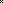
\includegraphics[width=\textwidth]{images/data_set/3x3_cross.png}
        \caption{Cross}
    \end{subfigure}
    \begin{subfigure}[b]{0.1\textwidth}
        \centering
        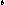
\includegraphics[width=\textwidth]{images/data_set/5x5_flame.png}
        \caption{Flame}
    \end{subfigure}
    \begin{subfigure}[b]{0.1\textwidth}
        \centering
        
\includegraphics[width=\textwidth]{images/data_set/8x8_jellyfish.png}
        \caption{Jellyfish \cite{8x8-src}}
    \end{subfigure}
    \begin{subfigure}[b]{0.1\textwidth}
        \centering
        
\includegraphics[width=\textwidth]{images/data_set/8x8_candy.png}
        \caption{Candy \cite{8x8-src}}
    \end{subfigure}
    \begin{subfigure}[b]{0.1\textwidth}
        \centering
        
\includegraphics[width=\textwidth]{images/data_set/10x10_shield.png}
        \caption{Shield \cite{10x10-src}}
    \end{subfigure}
    \begin{subfigure}[b]{0.1\textwidth}
        \centering
        
\includegraphics[width=\textwidth]{images/data_set/10x10_dog.png}
        \caption{Dog \cite{10x10-src}}
    \end{subfigure}
    \begin{subfigure}[b]{0.1\textwidth}
        \centering
        
\includegraphics[width=\textwidth]{images/data_set/16x16_duck.png}
        \caption{Duck \cite{16x16-src_duck}}
    \end{subfigure}
    \begin{subfigure}[b]{0.1\textwidth}
        \centering
        
\includegraphics[width=\textwidth]{images/data_set/16x16_shrimp.png}
        \caption{Shrimp \cite{16x16-src_shrimp}}
    \end{subfigure}
    \begin{subfigure}[b]{0.1\textwidth}
        \centering
        
\includegraphics[width=\textwidth]{images/data_set/20x20_cherries.png}
        \caption{Cherries \cite{20x20-src}}
    \end{subfigure}
    \begin{subfigure}[b]{0.1\textwidth}
        \centering
        
\includegraphics[width=\textwidth]{images/data_set/20x20_potion.png}
        \caption{Potion \cite{20x20-src}}
    \end{subfigure}
    \begin{subfigure}[b]{0.1\textwidth}
        \centering
        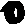
\includegraphics[width=\textwidth]{images/data_set/25x25_tape.png}
        \caption{Tape \cite{25x25-src}}
    \end{subfigure}
    \begin{subfigure}[b]{0.1\textwidth}
        \centering
        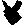
\includegraphics[width=\textwidth]{images/data_set/25x25_lighter.png}
        \caption{Lighter \cite{25x25-src}}
    \end{subfigure}
    \begin{subfigure}[b]{0.2\textwidth}
        \centering
        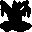
\includegraphics[width=\textwidth]{images/data_set/32x32_ghost.png}
        \caption{Ghost \cite{32x32-src}}
    \end{subfigure}
    \begin{subfigure}[b]{0.2\textwidth}
        \centering
        
\includegraphics[width=\textwidth]{images/data_set/32x32_demon.png}
        \caption{Demon \cite{32x32-src}}
    \end{subfigure}
    \begin{subfigure}[b]{0.2\textwidth}
        \centering
        
\includegraphics[width=\textwidth]{images/data_set/48x48_butcher.png}
        \caption{Butcher \cite{48x48-src_butcher}}
    \end{subfigure}
    \begin{subfigure}[b]{0.2\textwidth}
        \centering
        
\includegraphics[width=\textwidth]{images/data_set/48x48_ranger.png}
        \caption{Ranger \cite{48x48-src_ranger}}
    \end{subfigure}
    \begin{subfigure}[b]{0.4\textwidth}
        \centering
        
\includegraphics[width=\textwidth]{images/data_set/64x64_orc.png}
        \caption{Orc \cite{64x64-src_orc}}
    \end{subfigure}
    \begin{subfigure}[b]{0.4\textwidth}
        \centering
        
\includegraphics[width=\textwidth]{images/data_set/64x64_swordsman.png}
        \caption{Swordsman \cite{64x64-src_swordsman}}
    \end{subfigure}
    \caption{Zestaw danych}
\end{figure}
